\documentclass[../../main.tex]{subfiles}
\begin{document}

\begin{flushright}
\footnotesize\textit{【自動文字起こし・要確認】}
\end{flushright}

{\bf [解]} $C = \cos\theta, S = \sin\theta$ とおく. $x_1 = 1, y_1 = 0$ である $\dots \text{①}$. $A_n = \vec{a} \cdot \vec{OP_n}$, $B_n = \vec{b} \cdot \vec{OP_n}$ とすると,
\begin{align}
\vec{OP_{n+1}} &= 4(\vec{OP_n} - A_n \vec{a}) - 4(B_n - A_n \vec{a} \cdot \vec{b}) \vec{b} \quad \dots \text{②}
\end{align}
であり,
\begin{align}
A_n &= C x_n + S y_n, \\
B_n &= \dfrac{1}{2}(\sqrt{3} x_n + y_n), \\
\vec{a} \cdot \vec{b} &= \dfrac{1}{2}(\sqrt{3} C + S) \quad \dots \text{③}
\end{align}
より, $T = \vec{a} \cdot \vec{b}$ とおいて, ②から
\begin{align}
x_{n+1} &= (4 - 4C^2 - 3 + 2\sqrt{3}CT) x_n + (-4SC - \sqrt{3} + 2\sqrt{3}ST) y_n \\
&= (1 - C^2 + \sqrt{3}SC) x_n + (-SC - \sqrt{3}C^2) y_n \\
&= S(S + \sqrt{3}C) x_n - C(S + \sqrt{3}C) y_n \quad \dots \text{④} \\
y_{n+1} &= (-4CS - \sqrt{3} + 2CT) x_n + (4 - 4S^2 - 1 + 2ST) y_n \\
&= (-\sqrt{3}S^2 - 3CS) x_n + (3C^2 + \sqrt{3}CS) y_n \\
&= -\sqrt{3} S(S + \sqrt{3}C) x_n + \sqrt{3} C(S + \sqrt{3}C) y_n \quad \dots \text{⑤}
\end{align}
ここで, $\alpha = S(S + \sqrt{3}C), \ \beta = C(S + \sqrt{3}C)$ とすると,
\begin{align}
\begin{cases}
x_{n+1} = \alpha x_n - \beta y_n \\
y_{n+1} = -\sqrt{3} (\alpha x_n - \beta y_n)
\end{cases}
\quad \dots \text{①'}
\end{align}
だから, $y_{n+1} = -\sqrt{3} x_{n+1} \ (n \ge 1)$ なので,
\begin{align}
x_{n+1} &= (\alpha + \sqrt{3}\beta) x_n \quad (n \ge 2)
\end{align}
くり返し用いて,
\begin{align}
\begin{cases}
x_n = (\alpha + \sqrt{3}\beta)^{n-2} x_2 & (n \ge 2) \\
y_n = -\sqrt{3} (\alpha + \sqrt{3}\beta)^{n-2} x_2 & (n \ge 2)
\end{cases}
\quad \dots \text{⑦}
\end{align}
ここで, ①'から $x_2 = \alpha x_1 = \alpha$ だから, ①'から
\begin{align}
\begin{cases}
x_n = \alpha (\alpha + \sqrt{3}\beta)^{n-2} \\
y_n = -\sqrt{3}\alpha (\alpha + \sqrt{3}\beta)^{n-2}
\end{cases}
\quad (n \ge 2) \quad \dots \text{⑦'}
\end{align}
したがって, 数列 $\{x_n\}, \{y_n\}$ が収束する条件は,
\begin{align}
-1 < \alpha + \sqrt{3}\beta \le 1 \quad \text{or} \quad \alpha = 0
\end{align}
である. $\alpha, \beta$ に値を代入して
\begin{align}
-1 < (S + \sqrt{3}C)^2 \le 1 \quad \text{or} \quad S = 0 \text{ or } S + \sqrt{3}C = 0
\end{align}
\begin{align}
\iff -1 \le S + \sqrt{3}C \le 1 \quad \text{or} \quad S = 0 \quad \dots \text{⑧}
\end{align}
ここで, $S + \sqrt{3}C = 2 \sin\left(\theta + \dfrac{\pi}{3}\right)$ だから, $-1 \le S + \sqrt{3}C \le 1 \iff -\dfrac{1}{2} \le \sin\left(\theta + \dfrac{\pi}{3}\right) \le \dfrac{1}{2}$ に注意して,
\begin{align}
⑧ &\iff \dfrac{5}{6}\pi \le \theta + \dfrac{\pi}{3} \le \dfrac{7}{6}\pi, \ \dfrac{11}{6}\pi \le \theta + \dfrac{\pi}{3} \le \dfrac{13}{6}\pi \quad \text{or} \quad \theta = 0, \pi \\
&\iff \dfrac{1}{2}\pi \le \theta \le \dfrac{5}{6}\pi \quad \text{or} \quad \dfrac{3}{2}\pi \le \theta \le \dfrac{11}{6}\pi \quad \text{or} \quad \theta = 0, \pi
\end{align}
だから, ①'に注意して, $\sin\left(\theta + \dfrac{\pi}{3}\right) = \pm \dfrac{1}{2} \iff \theta = \dfrac{1}{2}\pi, \dfrac{5}{6}\pi, \dfrac{3}{2}\pi, \dfrac{11}{6}\pi$ より

$1^\circ$ $\dfrac{1}{2}\pi < \theta < \dfrac{5}{6}\pi, \ \dfrac{3}{2}\pi < \theta < \dfrac{11}{6}\pi, \ \theta = 0, \pi$ の時
$x_n, y_n$ 共に 0 に収束.

$2^\circ$ $\theta = \dfrac{1}{2}\pi, \dfrac{5}{6}\pi, \dfrac{3}{2}\pi, \dfrac{11}{6}\pi$ の時
$x_n \to \alpha, \ y_n \to -\sqrt{3}\alpha$ となるから, $\alpha = S(S + \sqrt{3}C)$ から,
$\theta = \dfrac{1}{2}\pi, \dfrac{3}{2}\pi$ の時, $x_n \to 1, \ y_n \to -\sqrt{3}$
$\theta = \dfrac{5}{6}\pi, \dfrac{11}{6}\pi$ の時, $x_n \to -\dfrac{1}{2}, \ y_n \to \dfrac{\sqrt{3}}{2}$
である.

以上まとめて,
\begin{align}
\begin{cases}
\theta = 0, \ \dfrac{1}{2}\pi < \theta < \dfrac{5}{6}\pi, \ \theta = \pi, \ \dfrac{3}{2}\pi < \theta < \dfrac{11}{6}\pi \text{ の時}, & (x_n, y_n) \longrightarrow (0, 0) \\
\theta = \dfrac{1}{2}\pi, \ \dfrac{3}{2}\pi & (x_n, y_n) \longrightarrow (1, -\sqrt{3}) \\
\theta = \dfrac{5}{6}\pi, \ \dfrac{11}{6}\pi & (x_n, y_n) \longrightarrow \left(-\dfrac{1}{2}, \dfrac{\sqrt{3}}{2}\right)
\end{cases}
\end{align}

\begin{figure}[htb]
\centering
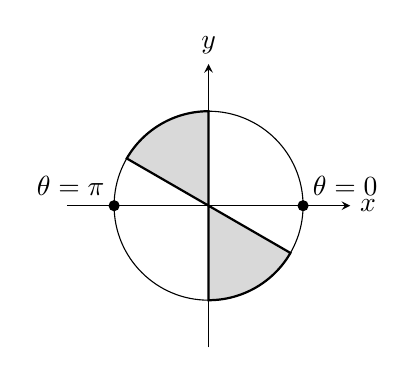
\begin{tikzpicture}[scale=1.2, >=stealth]
\draw[->] (-1.5,0) -- (1.5,0) node[right] {$x$};
\draw[->] (0,-1.5) -- (0,1.5) node[above] {$y$};
\draw (0,0) circle (1);
\draw[thick, fill=gray!30] (0,0) -- (90:1) arc (90:150:1) -- cycle;
\draw[thick, fill=gray!30] (0,0) -- (270:1) arc (270:330:1) -- cycle;
\filldraw (1,0) circle (1.5pt) node[above right] {$\theta=0$};
\filldraw (-1,0) circle (1.5pt) node[above left] {$\theta=\pi$};
\end{tikzpicture}
\caption{$(x_n, y_n)$が$(0,0)$に収束する$\theta$の範囲（斜線部）}
\end{figure}

\newpage

\end{document}
